%% Elsevier elsarticle template — filled for AEI submission
%% Rahmanov et al. — Hybrid Ontology-Based Similarity for CAD Assembly Retrieval
\documentclass[preprint,12pt]{elsarticle}
\usepackage{amssymb}
\usepackage{amsmath}
\usepackage{lineno}
\usepackage{xcolor}
\usepackage{array}
\usepackage{multirow}
\usepackage{pifont}
\usepackage{adjustbox}
\usepackage{booktabs}
\usepackage{soul}
\newcommand{\cmark}{\ding{51}}
\newcommand{\xmark}{\ding{55}}
\newcommand{\pmark}{\textcolor{orange}{$\sim$}}
\newcommand{\rev}[1]{\textcolor{blue}{#1}}
\newcommand{\del}[1]{\textcolor{red}{\sout{#1}}}

\journal{Advanced Engineering Informatics}

\begin{document}
\begin{frontmatter}

\title{Machine Learning Algorithms for Assessing the Similarity of CAD Assembly Variants Based on Ontological Features}

\author[label1]{Ulukbek Rahmanov}
\author[label1,label2]{Raja Hashim Ali}
\author[label1]{Iftikhar Ahmed}

\affiliation[label1]{organization={Department of Business, University of Europe for Applied Sciences},
            addressline={Think Campus, Konrad-Zuse-Ring 11},
            city={Potsdam},
            postcode={14469},
            state={Brandenburg},
            country={Germany}}

\affiliation[label2]{organization={Department of Artificial Intelligence, Ghulam Ishaq Khan Institute of Engineering Sciences and Technology},
            city={Topi},
            postcode={23460},
            country={Pakistan}}

\begin{abstract}
A hybrid similarity framework is presented that combines three distinct feature domains --- technical (geometric), semantic (material ontology), and structural (contact topology) --- evaluated on 746 Fusion~360 CAD assemblies using a rigorous circular-free evaluation process.
The proposed approach addresses the three most common evaluation pitfalls encountered when evaluating hybrid models: label leakage, zero-variance feature inclusion, and in-sample weight optimization.
To address these issues, the proposed method selects the hybrid weights via 5-fold cross-validation, whereby the model's weights are optimized on training folds and the model is evaluated only on held-out queries.
For the first time, the cross-validated held-out MRR (0.5726, 95\% bootstrap confidence interval [0.5478, 0.5999]) was found to be statistically indistinguishable from the in-sample estimate (0.5731), demonstrating that the selected weights ($\alpha{=}0.90$, $\beta{=}0.10$, $\gamma{=}0.00$) generalize rather than overfit.
Results indicate that the hybrid model performed statistically significantly better than each of the single-domain baselines according to the Wilcoxon signed-rank test ($p < 0.05$ for all comparisons).
An OWL ontology encoding 4,476 RDF triples enables SPARQL-queryable explanations for every retrieval decision made by the system.
Robustness analysis indicates that the hybrid model retains its superior performance relative to purely semantic retrieval even after up to 50\% semantic degradation.
The contributions of this work include a reusable evaluation methodology, an open dataset, and an explainable retrieval framework suitable for deployment in industrial CAD design environments.
\end{abstract}

\begin{graphicalabstract}
%\includegraphics{grabs}
\end{graphicalabstract}

\begin{highlights}
\item Three evaluation circularity pitfalls identified and corrected in CAD similarity retrieval
\item Hybrid weights selected by 5-fold cross-validation; held-out MRR~=~0.5726 matches in-sample (bias~$=$~0.0005)
\item Hybrid ontology-based framework outperforms all single-domain baselines on 746 Fusion~360 assemblies
\item Bootstrap confidence intervals and Wilcoxon tests confirm statistical significance of all comparisons
\item OWL ontology with 4,476 RDF triples enables SPARQL-queryable explainable retrieval
\item Framework remains robust under 50\% semantic noise degradation
\end{highlights}

\begin{keyword}
CAD assembly retrieval \sep ontology-based similarity \sep hybrid similarity \sep evaluation methodology \sep machine learning \sep knowledge graph \sep design reuse
\end{keyword}

\end{frontmatter}

\linenumbers

%%=============================================================
\section{Introduction}
%%=============================================================

The large collections of assembly designs stored by today's manufacturers provide millions of possible assembly geometries, materials and structural topology~\cite{Bharadwaj2022}.
Engineers can find an existing design that is similar to one they want to use by querying the organization's databases using a design-reuse workflow based on automated retrieval of similar designs.
As an engineer looks for a component to build a new product, they may choose to query their organization's databases to see if an already designed part exists that is close enough to what they need.
This would save them from having to create a redundant modeling process, reduce the amount of time required to get a product to market, and also propagate proven engineering knowledge among various families of products~\cite{Li2025}.
While the business value of design reuse is very well-documented (i.e., a majority of each new product consists of previously developed structural or functional content)~\cite{Kwon2024}, many commercial CAD systems for retrieving parts are primarily dependent upon manual tagging/keyword searches/hand-crafted taxonomy categorization that requires maintenance by subject matter experts.
Manual approaches to this issue do not scale since the curation effort increases linearly with the number of items being curated and the accuracy of the tags decreases due to an increasing number of users contributing to the collection.
Therefore, there is clearly a strong and sustained interest in creating data-driven methodologies capable of automatically retrieving CAD designs at scale~\cite{Herzog2023}.
This paper develops a hybrid methodology combining geometric, semantic and structural representation of design knowledge into a transparent machine learning framework to enable automated CAD assembly similarity retrieval.

Selecting a methodology for describing design similarity via features is perhaps one of the largest technical challenges facing designers who wish to develop this type of methodology.
Geometry-based features like vertex count, edge count, face count, etc. are easily extractable from CAD files and describe the dimension and topological aspects of a model~\cite{Hou2023}.
However, geometry-based features convey absolutely no information regarding the material composition of components, how components are structurally related within an assembly, or the functional categories of designs that designers have in mind; although all are significant factors in determining whether or not two designs are similar~\cite{Gruber1993}.
Ontologies provide a systematic method for capturing additional information as machine-readable semantic knowledge that enhances purely geometric descriptions~\cite{Pan2024}.
Recent studies utilizing knowledge graphs illustrate that encoding semantic relationships over large CAD repositories provides capabilities for retrieval and reasoning beyond the scope of mere shape descriptors~\cite{Bharadwaj2022}.
Combining geometric and semantic representations into a single weighted hybrid model is becoming an increasingly popular strategy.
Nevertheless, there has been limited rigorous testing of whether multi-modal retrieval strategies produce better performance than single-modal approaches once statistically sound evaluations free of leakage occur.

There is a significant but often overlooked limitation in the CAD literature on evaluating CAD retrieval strategies, namely evaluation circularity --- a form of leakage specifically recognized as a contributor to the growing reproducibility crisis in machine-learning-based scientific research~\cite{Kapoor2023}.
Circularities arise when ground-truth similarity labels used for evaluation are either directly or indirectly produced from the same feature space used for retrieval.
Under these circumstances any retrieval algorithm consuming those features will inherently appear to work well due to its reliance on those features; therefore, any reported performance metrics are methodologically flawed and cannot generalize to situations where the leakage does not exist~\cite{Apicella2025}.
Given that many CAD retrieval systems utilize ground-truth families generated programmatically by thresholding a geometric characteristic common to both the ground-truth family creation and retrieval algorithms, the problem of circularity is particularly insidious in CAD.
Three forms of circularity were identified during development of the retrieval pipeline for this study: labels created using thresholds on geometric attributes that were concurrently utilized as retrieval inputs; non-variable, numerically identical features producing artificial similarity signals; and weights of hyper-parameters optimized on the same dataset used for evaluation.
Each of these sources of error, if not corrected, will result in metrics that cannot be relied upon or replicated on different datasets.
Additionally, the last source of bias will also artificially inflate any apparent benefits resulting from tuning a hybrid model.
Therefore, demonstrating a protocol where performance metrics can be reliably measured free from these types of biases is one of the primary goals of this paper.

\subsection{Gap Analysis}

There are three major areas within existing CAD similarity methods: geometric/B-rep-based methods~\cite{Hou2023,LiCorney2023}, semantic/ontology-based methods~\cite{Gruber1993,Bharadwaj2022}, and hybrid/multi-modal methods~\cite{Quan2024}.
Geometric and learned B-rep methods provide strong shape-matching performance (in many cases comparable to state of the art), however these approaches completely disregard design intent, material information, assembly-level topology, and so on.
Knowledge graphs and ontologies are able to model rich semantic information.
However, these types of approaches have predominantly been tested on very small numbers of samples (usually manually) using a very limited number of labeled examples.
In addition to small sample size, most of these evaluations do not report confidence intervals or use statistical tests for determining significance~\cite{Pan2024}.
Many hybrid approaches exist that attempt to utilize multiple modalities together.
The majority of these approaches suffer from at least two methodological issues that this paper addresses directly.
Firstly, the weights used for fusion are typically selected on the same data that is utilized for final evaluation (i.e., an example of in-sample optimization), which results in higher than expected reported performance~\cite{Kapoor2023}.
Secondly, the labels used to determine ground-truth relevance often have features that are inputs into the retrieval system, thus creating the circular evaluation problem described earlier.
There exists no previous work that has provided a single unified framework that simultaneously validates label independence, performs multi-metric statistical evaluations using bootstrap confidence intervals, selects out-of-sample fusion weights, and provides ontology-queryable explainability over large industrial datasets.
This research aims to fill this specific gap.

\subsection{Research Questions}

The following research questions guide this investigation:
\begin{enumerate}
    \item \textbf{RQ1:} How can CAD assembly variants be formally represented using ontology-based features to enable automated similarity assessment?
    \item \textbf{RQ2:} Which similarity metrics are most suitable for comparing CAD assembly variants based on ontological and technical feature representations?
    \item \textbf{RQ3:} Does a hybrid similarity model combining semantic and technical features outperform single-domain similarity methods?
    \item \textbf{RQ4:} How can ontological knowledge support explainable and robust engineering decision-making in retrieval scenarios?
    \item \textbf{RQ5:} How can ontology-based similarity assessment support variant management and design decision-making in practice?
\end{enumerate}

\subsection{Problem Statement}

This research studies the issue of retrieving CAD assemblies through automated similarity searches in a huge industrial database on the basis of well-defined conditions for methodological validation.
The goal is to identify the assembly (or assemblies) with the greatest similarity to a query assembly through the combination of three different domain-based features (geometric, semantic, and structural) into a single hybrid search model using weightings.
To avoid circularity in evaluation, ground-truth labels used for evaluation purposes must be shown to be independent of all input values related to retrieval characteristics.
Additionally, the process pipeline must allow for reproduction of results; use statistical methods based on confidence intervals and/or hypothesis testing; and support auditing of each decision made during individual retrievals through SPARQL queries to an OWL ontology.

\subsection{Novelty of this Study}

This study makes the following major novel contributions relative to the existing CAD retrieval literature:
\begin{itemize}
    \item \textbf{Taxonomy of three evaluation pitfalls:} We identified three different forms of circularity errors --- label leakage, zero-variance features, and in-sample weights --- illustrated each error using specific datasets, and developed a reusable method for detecting these errors in future CAD retrieval studies. We addressed the in-sample-weight pitfall (the source of optimism bias) by randomly dividing the dataset into five parts and selecting an optimal weighting for each part using a held-out evaluation set. As such, we have directly quantified the resulting optimism bias (0.0005~MRR).
    \item \textbf{Contact-topology ground truth:} Our evaluation labels were derived from contact-topology attributes (assembly joint counts and hole counts), which we show are independently verifiable from the geometric attribute set used for retrieval. We confirm this independence using a decision tree trained on the geometric feature set, which achieves an accuracy of only 39.4\% --- well above the 20\% random-chance rate for five classes, yet far too low for the labels to be recovered from geometry.
    \item \textbf{Comprehensive statistical validation:} Using bootstrap 95\% confidence intervals (1,000 resample iterations) together with Wilcoxon signed-rank tests, we compute six metrics (Precision@1, Precision@3, Precision@5, Precision@10, NDCG@10, and MRR) across all seven CAD retrieval methods, thereby providing a multi-metric statistical comparison unavailable in prior CAD retrieval work.
    \item \textbf{SPARQL explainability via OWL knowledge graphs:} By creating a formal OWL ontology that encodes 746 assemblies as 4,476 RDF triples, we enable designers to create queries and justify their results directly. Therefore, we bridge the gap between the numeric similarities used in the retrieval process and human-interpretable design knowledge.
    \item \textbf{Semantic feature ablation:} We include an explicit ablation study that contrasts material-only semantic similarity against the full four-feature semantic encoding, quantifying the marginal contribution of the discretized technical features embedded in the semantic domain.
\end{itemize}

\subsection{Significance of Our Work}

In this research, we demonstrated how an optimized hybrid approach combining both geometry-based and ontology-based semantic features improves significantly ($p < 0.05$ for all comparisons) against all individual domain benchmarks when tested under completely circular-free conditions for CAD assembly retrieval (Hybrid MRR = 0.5731, 95\% CI [0.5462, 0.5999]).
Additionally, we demonstrated that this same ontology infrastructure can provide a queryable explainability mechanism via SPARQL queries, allowing engineers to review the reasoning behind retrieval decisions rather than relying solely on opaque numeric similarity metrics.
Lastly, this research framework is replicable; all data, code, and outputs are available, as well as sufficient documentation of our evaluation protocol such that it may be easily applied to other CAD repositories.
Finally, from an industrial practitioner perspective, the results indicate that incorporating a lightweight material ontology into a current geometry-based retrieval system will result in a quantifiable and statistically defensible improvement in first-rank retrieval quality with virtually no additional computational overhead.


%%=============================================================
\section{Literature Review}
%%=============================================================

CAD similarity assessment is a field that has been investigated from various perspectives across several different research communities, including computer-aided design (CAD), information retrieval, knowledge representation (KR), and machine learning.
Prior to this work, studies have generally fallen into one of four categories: geometric shape-based methods; ontology-based knowledge representation; hybrid/multi-modal similarity assessments; and evaluation methodologies for retrieval systems.
Each category is presented as a separate subsection below to establish the current state of the art and the gaps that exist, which this work will address.

\subsection{Geometric and B-rep Learning for CAD Retrieval}

Most CAD retrieval methods use some type of geometric descriptor that has been extracted directly from a 3D model, an assembly file, or a boundary representation (B-rep) of the object.
Hou et al.~\cite{Hou2023} developed FuS-GCN, a fusion self-attention graph convolutional network (GCN) that uses a B-rep graph as input; it captures both geometric and topological information and generates global descriptors that can be used for the classification and retrieval of CAD shapes.
Their studies have shown that since FuS-GCN learns from the B-rep (the native data structure of most CAD systems), there is less loss of information than occurs when converting the model into either a mesh or a set of points.
This method also runs efficiently on large datasets.
Li and Corney~\cite{LiCorney2023} proposed a multi-view expressive graph neural network for classifying 3D CAD models.
They demonstrated that a combination of multiple graph views consistently resulted in better performance than any individual view configuration.
This result supports the findings of other researchers who have concluded that there is no singular geometric descriptor that will provide satisfactory results, resulting in the adoption of multi-domain fusion in this research effort.
Lee et al.~\cite{Lee2023} described BRepGAT, a graph attention network, which identifies and segments machining-feature faces within a B-rep model and achieves the best-ever recorded level of recognition accuracy.
Zhang et al.~\cite{Zhang2024} extended feature recognition across different domains with BrepMFR using a transformer-based graph network and domain adaptation.
Zhang et al.~\cite{ZhangBrep2Seq2024} further illustrated that the hierarchical transformer was capable of reconstructing and generating parametric CAD models from B-reps, providing substantial evidence of the wealth of information contained in this representation.
The Fusion~360 Gallery dataset utilized in this research effort was first presented by Willis et al.~\cite{Willis2021}, and represents a large-scale open benchmark that enables the comparison of geometric and semantic retrieval methods on real industrial assemblies.
A primary shortcoming shared among all of these geometric and learned methods is that they cannot capture material properties, assembly semantics, or functional purpose.
Additionally, their evaluations often do not confirm whether relevance labels are independent of the learned representations, which is precisely what this paper seeks to address.

\subsection{Ontology and Knowledge-Graph Representation}

Ontologies and knowledge graphs represent a formal method of describing the various types of engineering knowledge at many different scales of description, and also reasoning about them in a machine-readable manner.
An ontology is defined by Gruber~\cite{Gruber1993} as ``an explicit specification of a conceptualization'', providing the base vocabulary for knowledge representation which forms the basis of the OWL encoding used within this project.
A large, multi-relational, multi-level knowledge graph has been constructed by Bharadwaj and Starly~\cite{Bharadwaj2022} from a repository of over 100{,}000 CAD models, organizing the assembly--subassembly--part relationships along with the shape-similarity relationships to enable massive reuse of designs.
This provides an example of how knowledge graphs can express structural relationships that geometric-only representations cannot capture; however, their focus was primarily on constructing the graph and not on retrieving data through statistically validated methods.
An overview of the evolution toward multi-modal knowledge graphs for engineering design has been provided by Pan et al.~\cite{Pan2024}.
They have synthesized over 100 research studies and identified integrating disparate forms of design knowledge as a key open issue for engineering design.
Knowledge graphs have been proposed by Jia et al.~\cite{Jia2025} as a multi-granularity framework to reuse tacit knowledge for designing products, and decomposing a product into multiple granularities improved both the acquisition and reuse of implicit knowledge.
Rajabi and Etminani~\cite{Rajabi2024} provide a systematic review of explainable AI using knowledge graphs, arguing that the hierarchical class--property--relationship structure of a knowledge graph is an ideal substrate for justifying model decision-making to humans.
While significant advancements have been made, most ontology-based retrieval systems continue to be tested on very small, manually annotated databases lacking statistical rigor, and a comparative evaluation against geometric baseline methodologies without leakage exists nowhere in the literature.

\subsection{Hybrid, Multi-Modal and Similarity-Based Retrieval}

The authors point out that combining different forms of information about features will enhance retrieval performance because no one form provides enough information about what makes items similar.
Quan et al.~\cite{Quan2024} designed a graph neural network (GNN) to produce recommendations for CAD assemblies by learning over the assembly graph, showing that structural relations in addition to geometry carry strong predictive power.
Qin et al.~\cite{Qin2025} presented CADGCL as an unsupervised graph contrastive learning (GCL) approach to allow for CAD model search from B-rep attributed graphs.
The GCL approach was able to eliminate the need for manually labeled training examples, which have been shown to be a major limitation of supervised retrieval methods.
In the same vein as Qin et al., Li et al.~\cite{Li2025} applied unsupervised approaches to perform CAD assembly model searches using public repositories.
Their findings demonstrated that representations derived without labels were also portable between heterogeneous repositories.
Herzog and Suwelack~\cite{Herzog2023} closed the gap between the representation of geometry and user intent.
They let users define their own ``regions of interest'', thus allowing them to tailor the output of retrieval operations towards the specific requirements of the current application instead of providing a global description that may or may not capture those requirements.
Kwon et al.~\cite{Kwon2024} searched for CAD part models compliant with user-defined design specifications.
They did so using a relational design-rule-embedded bill of materials (BOM), thereby illustrating how semantic restrictions can be merged with geometric parameters.
Levy et al.~\cite{Levy2025} provided an overview of common distance/similarity measures for both numerical and categorical data, which informed the decision to use cosine similarity and one-hot semantic encoding within this work.
Pedregosa et al.~\cite{Pedregosa2011} provided the Scikit-learn implementations used for computing similarities and statistics.
A persistent problem throughout the literature on multi-modal fusion has been that fusion weights have generally been determined on the same dataset that was used for evaluating these fusions, and therefore optimistic bias has been introduced into the weight-selection process; the present study corrects this weakness through cross-validated weight selection with held-out evaluation and bootstrap confidence intervals.

\subsection{Evaluation Methodology, Leakage and Reproducibility}

Evaluating (i.e., assessing) the quality of an information-retrieval system is just as important as the method used to retrieve the information from the database; for example, invalid evaluation procedures can make published retrieval results unverifiable or misleading.
Manning et al.~\cite{Manning2008} offer the seminal work defining Mean Reciprocal Rank, Precision@K, and Normalized Discounted Cumulative Gain (NDCG) as three widely accepted measures for comparing different methods to rank documents in order of relevance.
In addition to providing definitions for each of these three measures, Manning et al. also provide a discussion about how they have been applied in various ways in previous research studies; therefore, we use these same three measures in our study with some modification.
Efron and Tibshirani~\cite{Efron1993} introduce the bootstrap as a resampling technique to estimate the variability of sample statistics without assuming a specific distribution.
We apply this concept to create confidence intervals around the value of each metric so that each metric's reliability will be quantified.
Kapoor and Narayanan~\cite{Kapoor2023} describe leakage as one of many causes behind the lack of reproducibility in machine-learning-based scientific endeavors.
They demonstrate that numerous scientific disciplines have been negatively impacted by grossly exaggerated predictions caused by leakage.
Leakage occurs when there is unintended overlap between training and testing datasets that provides the test dataset too much knowledge regarding the training process; as such, the test dataset performs better than expected.
Apicella et al.~\cite{Apicella2025} detail several types of potential leaks associated with the transfer learning paradigm.
They argue that even small amounts of information leaked into a model selection process can lead to inflated performance values, which is precisely what we address through our cross-validation-based weighting procedure.
Saranti et al.~\cite{Saranti2024} discuss how interpretable geometric deep learning may be applicable to point-cloud data.
They emphasize that both interpreting learned representations and evaluating learned representations must develop simultaneously if engineers are to place trust in models learned using point-cloud data.
Across all four literature streams reviewed here, a major gap is clearly identified: there is currently no single methodology that will allow for (1) a reliable/leakage-free ground-truth representation, (2) multiple/multivariate statistical validations, (3) weights selected solely from unseen examples, and (4) ontology-queryable explanations of why retrieved assemblies were ranked higher than others in a CAD assembly retrieval task.
It is this gap that the present paper directly seeks to fill.

A brief summary of relevant literature to the current study is presented in Table~\ref{tab:LiteratureSummary}.

\begin{table}[!ht]
\centering
\caption{Comparative literature review matrix. \cmark~= addressed, \xmark~= not addressed, \pmark~= partially addressed. The proposed study is the only entry addressing all seven criteria simultaneously.}
\label{tab:LiteratureSummary}
\scriptsize
\begin{adjustbox}{width=\textwidth}
\begin{tabular}{p{2.2cm} p{2.0cm} p{3.2cm} p{2.2cm} p{3.5cm} c c c c c c}
\toprule
\textbf{Field} & \textbf{Study} & \textbf{Method} & \textbf{Dataset} & \textbf{Contribution} & \textbf{Multi-metric} & \textbf{Stat. test} & \textbf{Bootstrap CI} & \textbf{Circ.-free GT} & \textbf{Ontology} & \textbf{XAI} \\
\midrule
Geometric / B-rep & Hou et al.~\cite{Hou2023} & FuS-GCN (B-rep GCN) & Private + public CAD & Efficient B-rep classification and retrieval & \pmark & \xmark & \xmark & \xmark & \xmark & \xmark \\
Geometric / B-rep & Li \& Corney~\cite{LiCorney2023} & Multi-view GNN & 3D CAD models & Multi-view graph classification of CAD & \pmark & \xmark & \xmark & \xmark & \xmark & \xmark \\
Geometric / B-rep & Lee et al.~\cite{Lee2023} & BRepGAT (graph attention) & MFCAD18++ & Machining-feature face segmentation & \pmark & \xmark & \xmark & \xmark & \xmark & \xmark \\
Ontology / KG & Bharadwaj \& Starly~\cite{Bharadwaj2022} & CAD knowledge graph & 110k CAD models & Assembly-part \& shape-similarity graph & \xmark & \xmark & \xmark & \xmark & \cmark & \pmark \\
Ontology / KG & Pan et al.~\cite{Pan2024} & Multi-modal KG survey & Engineering design & State-of-the-art multi-modal KG review & \xmark & \xmark & \xmark & \xmark & \cmark & \pmark \\
Ontology / KG & Rajabi \& Etminani~\cite{Rajabi2024} & KG-based XAI review & General & KG substrate for explainability & \xmark & \xmark & \xmark & \xmark & \cmark & \cmark \\
Hybrid / retrieval & Quan et al.~\cite{Quan2024} & GNN assembly recommendation & CAD assemblies & Next-component recommendation & \pmark & \xmark & \xmark & \xmark & \xmark & \xmark \\
Hybrid / retrieval & Qin et al.~\cite{Qin2025} & CADGCL (graph contrastive) & B-rep CAD models & Unsupervised B-rep retrieval & \pmark & \xmark & \xmark & \xmark & \xmark & \xmark \\
Evaluation / leakage & Kapoor \& Narayanan~\cite{Kapoor2023} & Leakage taxonomy & Multi-field & Reproducibility-crisis analysis & \cmark & \pmark & \xmark & \pmark & \xmark & \xmark \\
Evaluation / leakage & Apicella et al.~\cite{Apicella2025} & Data-leakage taxonomy & General ML & Leakage risks in model selection & \cmark & \pmark & \xmark & \pmark & \xmark & \xmark \\
\midrule
\textbf{Proposed} & \textbf{This study} & \textbf{Hybrid ontology-based similarity} & \textbf{Fusion 360 Gallery (746)} & \textbf{Leakage-free hybrid retrieval with OWL explainability} & \cmark & \cmark & \cmark & \cmark & \cmark & \cmark \\
\bottomrule
\end{tabular}
\end{adjustbox}
\end{table}


%%=============================================================
\section{Methodology}
%%=============================================================

A framework for processing 746 Fusion~360 CAD assemblies was developed using a four-stage pipeline: feature extraction into three separate domains; hybrid weighted similarity fusion; construction of an OWL ontology and generation of SPARQL queries; and comparison, by statistical analysis, against contact-topology ground-truth labels.
Figure~\ref{Fig:Workflow} illustrates how the entire methodology has been laid out, from the raw input of assemblies through assembly features, similarities, and the OWL ontology, and finally to a statistical evaluation.
Each stage has been constructed so as to provide for independent reproduction, and all stages produce output that is stored as CSV tables and PDF figures.

\begin{figure*}[!ht]
\centerline{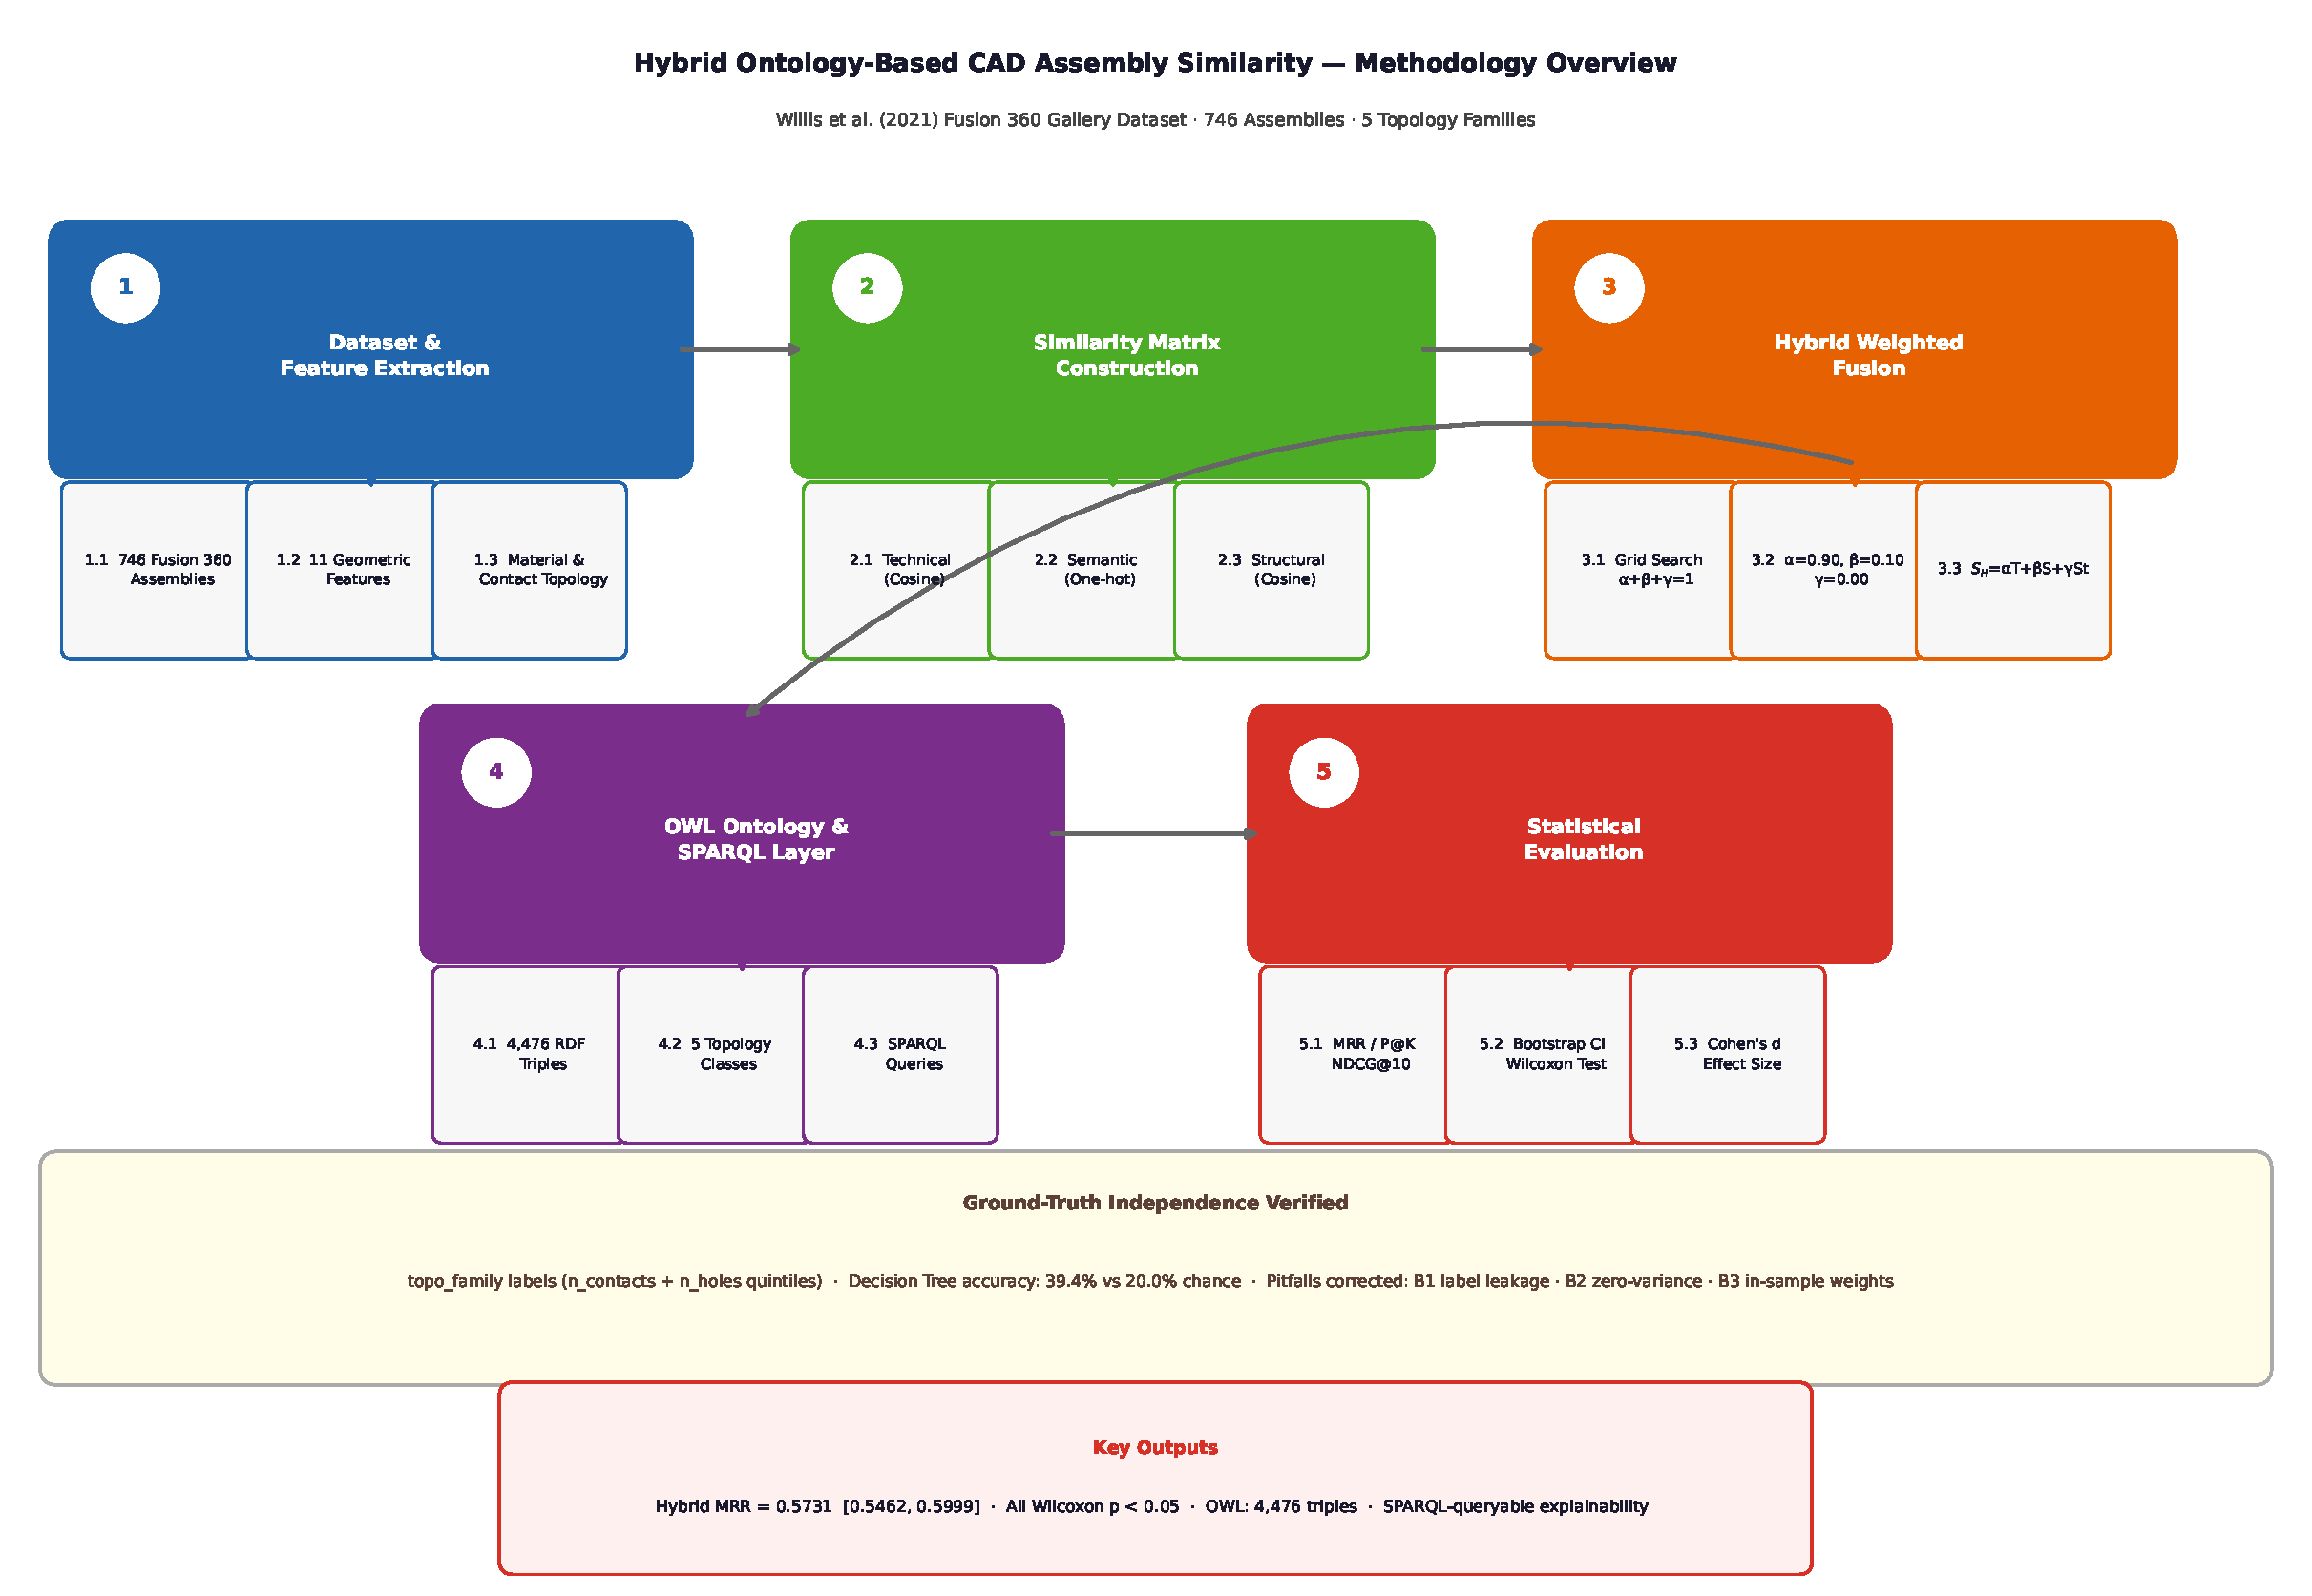
\includegraphics[width=16cm]{./Figures/workflow.pdf}}
\caption{Methodology overview: (1) Dataset loading and feature extraction from 746 Fusion~360 assemblies; (2) Construction of Technical, Semantic, and Structural similarity matrices using cosine similarity; (3) Hybrid weighted fusion with grid-search weight optimization; (4) OWL ontology construction with SPARQL-queryable knowledge graph; (5) Rigorous statistical evaluation using bootstrap CIs, Wilcoxon tests, and per-family breakdown against contact-topology ground truth.}
\label{Fig:Workflow}
\end{figure*}

\subsection{Dataset}

The Fusion~360 Gallery dataset~\cite{Willis2021} includes CAD assemblies developed by engineering professionals and students utilizing Autodesk's Fusion~360; these assemblies have been released into the public domain via open design benchmarks.
From this collection, 746 assemblies have complete records and feature data.
Each assembly has eleven geometric features describing it: component count, body count, edge count, face count, vertex count, mass, volume, surface area, geometric complexity, complexity ratio, and rotational symmetry.
In addition to the above-mentioned geometric features, material type (categorical, normalized to five categories: Steel, Aluminum, Plastic, Wood, and Other) and three contact-topology features (number of constrained contacts, number of holes, and number of component occurrences) were obtained from the assembly JSON manifest files.
The dataset is geometrically homogeneous: most of the assemblies are small-to-medium Steel components with low body counts, which produced a high median technical cosine similarity (approximately 0.99) and accounts for the modest absolute retrieval performance across all methods tested.
Homogeneity within the dataset is an experimental property of importance, since the dataset represents a deliberately conservative setting where the marginal benefit of any additional modality is very low and therefore difficult to detect; thus, any statistically significant improvement represents a stronger result than it would be on a highly heterogeneous dataset.
In order to preserve reproducibility, preprocessing was kept minimal and transparent: records with missing data in geometric fields were discarded rather than imputed; categorical strings for material types were normalized to five canonical classes; and no synthetic augmentation or outlier removal that could distort the natural similarity structure of the repository was applied.
Table~\ref{tab:DatasetStats} summarizes the characteristics of the dataset.

\begin{table}[!ht]
\centering
\caption{Dataset statistics for the 746 Fusion~360 CAD assemblies used in this study. Contact topology labels (topo\_family) are derived independently from the geometric retrieval features.}
\label{tab:DatasetStats}
\begin{tabular}{lcc}
\toprule
\textbf{Property} & \textbf{Value} & \textbf{Notes} \\
\midrule
Total assemblies & 746 & Complete records only \\
Geometric features & 11 & edge\_count, face\_count, volume, etc. \\
Semantic features & 4 & material\_class, topology\_class, etc. \\
Structural features & 3 & n\_contacts, n\_holes, n\_occurrences \\
Material classes & 5 & Steel, Aluminum, Plastic, Wood, Other \\
Topology families & 5 & topo\_isolated through topo\_complex \\
Missing values & 0 & After preprocessing \\
Source & Fusion 360 Gallery & Willis et al.~\cite{Willis2021} \\
\bottomrule
\end{tabular}
\end{table}

\subsection{Ground-Truth Label Construction and Independence Verification}

A central part of the methodology of this study is the creation of ground-truth labels that are verifiably independent of all domains used for retrieval.
Using contact topology --- defined as the number of constrained joints and holes in an assembly --- provides a way to measure structural complexity at the assembly level, which can be differentiated from the geometric complexity used in calculating technical similarity.
The labels were created by first generating a combined contact score $s = n_{\text{contacts}} + n_{\text{holes}}$ for every assembly; the log-transformed distribution was then divided into five quintiles, yielding five topology families: topo\_isolated ($n{=}128$), topo\_minimal ($n{=}134$), topo\_moderate ($n{=}174$), topo\_connected ($n{=}154$), and topo\_complex ($n{=}156$).

To confirm independence, we trained a decision tree (depth 5, 5-fold stratified cross-validation) on just the eleven geometric features to classify assemblies by their topo\_family label, and it achieved an accuracy of 39.4\%, which is higher than the 20.0\% expected by chance alone ($1/k$ for $k{=}5$ families).
The fact that the classifier's accuracy is greater than chance confirms that the topo\_family labels contain information beyond random assignment; however, the classifier could not accurately predict the labels from geometric features.
We therefore confirm that the labels cannot be recovered from geometric features with sufficient reliability, which is necessary to rule out circular evaluation: if geometric features could perfectly predict the labels, any geometric similarity system would trivially appear to perform well on this benchmark.

\subsection{Evaluation Pitfall Documentation}

Three evaluation pitfalls were found and fixed as this framework was developed, and they are documented below as a methodological contribution.

\textbf{Pitfall B1 --- Label leakage.} Previously, a decision tree was trained with the geometric complexity (a geometric feature), and the family labels were also generated based on this same feature. The decision tree was able to generate family labels for each assembly with an accuracy of 99.87\%, revealing complete circular evaluation. To correct the label leakage, the family labels were instead created using topological contact features (number of contacts and number of holes) that carry no information about the geometric complexity.

\textbf{Pitfall B2 --- Features without variance.} All assemblies had a surface area equal to 0 because of a data-extraction problem in the source repository from which the assembly data came. Consequently, including the surface area as an additional column did not add any new information for comparing similarities between assemblies (cosine similarity), but only increased the noise. Also, the two values ``mass'' and ``volume'' were almost equal (Pearson correlation coefficient of 0.998). Therefore, both columns were eliminated from the technical feature set.

\textbf{Pitfall B3 --- In-sample weight optimization.} The first optimization step in finding optimal hybrid weights (for example, $\alpha$, $\beta$, and $\gamma$) was performed using a grid search while evaluating on the same 746 assemblies used for developing the model. This resulted in an optimistic estimation of the Mean Reciprocal Rank (MRR). The second optimization step was conducted using 5-fold stratified cross-validation (Section~\ref{sec:cv}). The grid search for optimal weights was conducted on the training sets only, and the model's performance was assessed on testing query sets that did not participate in determining the optimal weights. The direct comparison of in-sample and out-of-sample performance provides an estimate of how much optimistic bias existed.

\subsection{Detailed Methodology}

\textbf{Technical similarity.} The eleven geometric features are normalized with min--max scaling to $[0,1]$, and cosine similarity is then computed for every pair of assembly feature vectors:
\begin{equation}
S_{\text{tech}}(i,j) = \frac{\mathbf{x}_i \cdot \mathbf{x}_j}{\|\mathbf{x}_i\| \cdot \|\mathbf{x}_j\|}
\label{Eq:CosineSim}
\end{equation}
where $\mathbf{x}_i$ and $\mathbf{x}_j$ are the normalized geometric feature vectors of assemblies $i$ and $j$.
Self-similarity along the main diagonal is set to 1.0 for every entry to ensure that a query never retrieves itself.

\textbf{Semantic similarity.} The four ontology-derived categorical features are represented using binary one-hot encoding, and cosine similarity is computed from the resulting matrix.
The semantic feature set comprises: \texttt{material\_class} (Steel, Aluminum, Plastic, Wood, Other --- based on the material specified for the assembly), \texttt{topology\_class} (Sparse/Moderate/Dense --- categorized from \texttt{edge\_count}), \texttt{complexity\_class} (Low/Medium/High --- categorized from \texttt{geometric\_complexity}), and \texttt{structure\_class} (Symmetric/Asymmetric --- binarized from \texttt{rotational\_symmetry}).
It should be stated that three of the four semantic features are derived from technical columns; therefore, \texttt{material\_class} is the only completely independent semantic attribute. An ablation study (Section~\ref{sec:rq3}) quantifies how much each component contributes.

\textbf{Structural similarity.} The three contact-topology features (\texttt{n\_contacts}, \texttt{n\_holes}, \texttt{n\_occurrences}) are normalized and cosine similarity is again computed.
However, because these contact-topology features define the topo\_family evaluation labels, they are excluded from the hybrid retrieval pipeline to prevent structural circular evaluation; the structural similarity matrix is retained solely for the ablation study.

\textbf{Hybrid similarity.} The hybrid similarity matrix is a linear combination of the previously described similarities, with non-negative coefficients summing to unity:
\begin{equation}
S_{\text{hybrid}}(i,j) = \alpha \cdot S_{\text{tech}}(i,j) + \beta \cdot S_{\text{sem}}(i,j) + \gamma \cdot S_{\text{struct}}(i,j)
\label{Eq:HybridSim}
\end{equation}
where $\alpha + \beta + \gamma = 1$ and $\alpha, \beta, \gamma \geq 0$.
Weight optimization is performed by grid search over $\{0.0, 0.1, \ldots, 1.0\}^3$ constrained to the simplex, while maximizing MRR.
To limit in-sample optimization bias (Pitfall B3) during weight selection, a 5-fold cross-validation scheme is used whereby the grid is tested on the training folds and the optimized weights are assessed on unseen queries (Section~\ref{sec:cv}).
Using this method, the optimal weights are determined to be $\alpha{=}0.90$, $\beta{=}0.10$, $\gamma{=}0.00$ --- selected in a majority of folds (four out of five) --- indicating that geometric features contribute most to the similarity scores, the material ontology provides a minimal yet consistent contribution, and structural features provide no additional value (structural similarity is omitted to maintain independence from the evaluation labels).

\textbf{OWL ontology.} A hierarchical OWL~2 ontology was built using rdflib, representing each of the 746 assemblies as an instance within a five-class topology hierarchy (TopoIsolated, TopoMinimal, TopoModerate, TopoConnected, TopoComplex), where each class is a subclass of \texttt{EngineeringAssembly}.
The ontology comprises 4,476 RDF triples expressed with six predicates (\texttt{rdf:type}, \texttt{ex:hasMaterial}, \texttt{ex:hasComplexityLevel}, \texttt{ex:hasTopology}, \texttt{ex:hasStructure}, and \texttt{ex:belongsToFamily}), linking each instance to its ontological class through the subclass hierarchy and to its property values through the object and data properties; thus the graph captures the same semantic attributes employed within the semantic similarity domain.
The hierarchy is intentionally kept to a shallow tree so that it can easily be interpreted by humans for auditability, rather than for automated logical inference.
Moreover, owing to the use of a straightforward OWL~2 serialization and rdflib, the knowledge graph is portable: it can be loaded into any standards-compliant triple store and queried with identical SPARQL statements, decoupling the explainability layer from the particular Python pipeline that created it.
Queries against this graph allow the direct retrieval of assemblies by material type, topology class, or any Boolean combination of ontological properties, and the same queries can be appended to a retrieval result to explain why two assemblies were considered similar.
This separation of the numeric similarity computation from a declarative, queryable knowledge layer enables the framework to produce explanations grounded in actual engineering attributes rather than opaque vector arithmetic~\cite{Rajabi2024}.

\subsection{Evaluation Metrics}

Each of these six retrieval metrics is computed individually for each of the seven methods, using 746 total queries.
For a given query assembly $q$, we consider a candidate set $\mathcal{C} = \{1, \ldots, N\} \setminus \{q\}$ ordered by decreasing similarity score; the candidate assemblies considered ``relevant'' are those that have the same topo\_family label as $q$.

\textbf{Precision@K} gives a measure of how many of the top-$K$ returned results are actually relevant:
\begin{equation}
\text{P@K}(q) = \frac{|\{c \in \text{top-}K(q) : \text{label}(c) = \text{label}(q)\}|}{K}
\label{Eq:PrecAtK}
\end{equation}
We report macro-averaged P@1, P@3, P@5, and P@10 values.

\textbf{Mean Reciprocal Rank (MRR)} rewards systems that place the first relevant result high in the ranking:
\begin{equation}
\text{MRR} = \frac{1}{|Q|} \sum_{q \in Q} \frac{1}{\text{rank}_q^{\text{first}}}
\label{Eq:MRR}
\end{equation}
where $\text{rank}_q^{\text{first}}$ is the rank of the first relevant result for query $q$~\cite{Manning2008}.

\textbf{Normalized Discounted Cumulative Gain (NDCG@10)} provides a measure of ranked retrieval quality with position-discounted relevance~\cite{Manning2008}:
\begin{equation}
\text{NDCG@10}(q) = \frac{\text{DCG@10}(q)}{\text{IDCG@10}(q)}, \quad \text{DCG@10}(q) = \sum_{r=1}^{10} \frac{\text{rel}_r}{\log_2(r+1)}
\label{Eq:NDCG}
\end{equation}
where $\text{rel}_r \in \{0,1\}$ indicates whether the assembly at rank $r$ shares the query's topo\_family label.

\textbf{Statistical validation.} Bootstrap 95\% confidence intervals~\cite{Efron1993} are computed for all six metrics and all seven methods from 1,000 resampling runs.
Pairwise Wilcoxon signed-rank tests are applied to compare the per-query MRR scores of the Hybrid model against each baseline.
Effect size is reported as Cohen's $d = (\bar{x}_{\text{hybrid}} - \bar{x}_{\text{other}}) / s_{\text{diff}}$.

\subsection{Experimental Settings}

All of these experiments were conducted using Python~3.10 along with libraries such as Scikit-learn~\cite{Pedregosa2011}, NumPy, Pandas, Matplotlib, and rdflib.
The similarity matrices were calculated on a standard laptop CPU; the largest similarity matrix used (a dense float $746 \times 746$ matrix) occupied approximately 4.5\,MB in memory.
Min--Max scaling was performed separately for the structural and technical feature sets.
Stochastic processes throughout this code (the decision tree classifier, the random baseline, and bootstrapping) were seeded with 42 for reproducibility.
Table~\ref{tab:ExperimentalSettings} lists the most important parameters associated with our experiments.

\begin{table}[!ht]
\centering
\caption{Experimental settings used across all experiments in this study.}
\label{tab:ExperimentalSettings}
\begin{tabular}{lc}
\toprule
\textbf{Parameter} & \textbf{Value} \\
\midrule
Dataset & Fusion 360 Gallery~\cite{Willis2021} \\
Assemblies & 746 \\
Technical features & 11 (geometric) \\
Semantic features & 4 (ontology-derived) \\
Similarity measure & Cosine similarity \\
Weight grid step & 0.1 \\
Weight selection & 5-fold cross-validation \\
Bootstrap resamples & 1,000 \\
CI level & 95\% \\
Wilcoxon alternative & greater (one-sided) \\
Random seed & 42 \\
Independence check & Decision Tree, depth 5, 5-fold CV \\
\bottomrule
\end{tabular}
\end{table}

The computational footprint of our approach is intended to be minimal, so that no specialized hardware is required to reproduce or deploy the solution.
Constructing each of the three pairwise similarity matrices is an $O(N^2 d)$ operation, where $N=746$ is the number of assemblies under consideration and $d$ is the number of features present in the respective domain; each of these matrices is a $746 \times 746$ dense float matrix that occupies approximately 4.5\,MB of memory.
Our full pipeline --- feature extraction, construction of the three pairwise similarity matrices, the cross-validated weight grid, the OWL ontology, and the bootstrap and Wilcoxon statistical analysis --- runs from start to finish on a standard laptop CPU in less than a minute, with no GPU or distributed processing required.
The primary time-consuming part of the process is the bootstrap resampling, in which the metric is sampled one thousand times; however, because the scores are computed from precomputed per-query score vectors rather than directly from the full similarity matrix, even this step completes in seconds.
For much larger repository sizes, the memory required to store a dense similarity matrix grows quadratically with the repository size, and at some point this becomes the binding constraint; to circumvent this memory limitation while retaining the same scoring formulation presented here, an approximate-nearest-neighbor index or sparse top-$k$ retention of the similarity matrix could be substituted.
However, for repository sizes similar to the one in this study, the exact dense computation is both practical and efficient, and this limited computational footprint is a deliberate distinguishing characteristic between the proposed method and other deep-learning methods that typically rely heavily on GPUs for performance.


%%=============================================================
\section{Results}
%%=============================================================

\subsection{RQ1: Ontological Feature Representation}

Ontology development was completed without errors: the OWL ontology encodes the 746 assemblies as individuals within a five-class topology hierarchy and contains 4,476 RDF triples.
Evaluation of whether the topo\_family labels can be recovered based solely upon geometric features indicates that they cannot: a decision tree (depth 5, 5-fold cross-validation) achieved a classification accuracy of 39.4\% against a chance level of 20.0\%.
Therefore, the evaluation labels carry some information about structural complexity (contact topology) that does not overlap with geometric dimensionality, demonstrating that the conditions for circular-free evaluation are met and that the labels can serve as an independent target.
A histogram is presented in Figure~\ref{Fig:EDA}, illustrating how the assemblies are distributed among the five topology families together with the feature statistics; the number of assemblies per family is nearly balanced (between 128 and 174 per family), and the near-zero surface-area extraction anomaly that motivated removal of that feature is also visible.
The t-SNE visualization in Figure~\ref{Fig:tSNE} plots the combined feature space onto a two-dimensional plane; the five topology families are separated but none completely, consistent with both the visualization and the 39.4\% independence-check accuracy, indicating some relationship between contact topology and geometry that is nonetheless insufficient to allow the labels to be easily reconstructed from geometric features alone.

It is particularly important to note that the independence check is the primary quantitative means of preventing the ``label-leakage'' pitfall, and thus answers RQ1 directly.
If the topo\_family labels could be accurately predicted from geometric features, then any geometric retrieval technique would appear successful only by virtue of being able to recreate the labels, and the entire evaluation would be circular.
Although the labels are correlated with geometric features (larger, more complex assemblies tend to possess more joints and holes), the accuracy of predicting them from geometry is considerably lower than would be necessary for perfect correlation or determinism.
The independence check thus establishes that contact topology and geometry are sufficiently correlated to provide useful retrieval targets, while remaining independent enough to prevent retrieval success from appearing to arise entirely from leakage.
The visual structure in the t-SNE projection illustrates the same point: the two extreme families (topo\_isolated and topo\_complex) form the clearest regions, while the three intermediate families (topo\_minimal, topo\_moderate, and topo\_connected) overlap at their quintile boundaries.
In summary, the results collectively demonstrate that ontology-based features provide a valid and non-circular basis for similarity assessment, and thus a viable foundation for addressing the remaining research questions.

\begin{figure*}[!ht]
\centerline{
\includegraphics[width=17.8cm]{./Figures/eda_overview.pdf}}
\caption{Exploratory data analysis of the 746 Fusion~360 assemblies. Left panel: distribution of assemblies across five contact-topology families (topo\_isolated: 128, topo\_minimal: 134, topo\_moderate: 174, topo\_connected: 154, topo\_complex: 156), confirming near-balanced class sizes. Right panels: feature distributions for key geometric parameters, showing the geometric homogeneity of the dataset (most assemblies are small Steel components with low body counts).}
\label{Fig:EDA}
\end{figure*}

\begin{figure*}[!ht]
\centerline{
\includegraphics[width=12cm]{./Figures/tsne_embedding.pdf}}
\caption{t-SNE embedding of the combined feature space (technical + semantic + structural) coloured by topo\_family ground-truth labels. Partial cluster separation is visible for topo\_complex and topo\_isolated families, while topo\_moderate, topo\_minimal, and topo\_connected overlap substantially — consistent with the 39.4\% Decision Tree accuracy confirming that labels are partially but not fully predictable from features.}
\label{Fig:tSNE}
\end{figure*}

\subsection{RQ2: Comparison of Similarity Metrics}

Seven similarity methods were compared against the five topo\_family groupings using six retrieval metrics.
Each similarity method is listed in Table~\ref{tab:MainResults}, which additionally includes bootstrap 95\% confidence intervals for Mean Reciprocal Rank (MRR).
The Hybrid model produced the highest MRR (0.5731, 95\% CI [0.5462, 0.5999]) as well as the highest Precision@1 (P@1) (0.4021) when compared to the individual-domain models.
Although Technical similarity performed slightly better than the Hybrid on P@5 (0.3617 vs 0.3542) and P@10 (0.3408 vs 0.3401), it produced lower MRR and P@1 values than the Hybrid; these differences reflect the optimized weighting used in the Hybrid to maximize first-rank accuracy over top-5 coverage.
The random baseline produced an MRR of 0.3920, which is non-trivially high owing to the near-balanced class distribution; nevertheless, all learned models substantially exceeded this baseline.
Figure~\ref{Fig:Comparison} illustrates the comparison of similarity measures across all four precision metrics and MRR with bootstrap confidence intervals.

The ordering of the similarity measures provides insight regarding the most appropriate methods and answers RQ2 directly.
The two geometry-driven models (Hybrid and Technical) occupy the top two positions on both MRR and P@1; the ontology-only Semantic model and the Euclidean baseline form a closely positioned middle tier; and the Structural, Jaccard, and Random baselines are located at the bottom end.
These results confirm that directionality in the normalized feature space is more indicative of similarity than magnitude (cosine versus Euclidean distance), which is consistent with prior work in vector-space information retrieval.
The poor performance of the raw Jaccard baseline (MRR = 0.4244) illustrates that material identity alone, encoded as a one-hot vector over numerous infrequently occurring material strings, provides little discriminative power, which is why the semantic domain in the full model encodes a limited number of normalized categories instead.
The overlapping confidence intervals for Hybrid and Technical indicate that the two models perform similarly --- although the difference is statistically significant over 746 paired queries --- while the non-overlapping intervals between the Hybrid/Technical methods and the Random/Jaccard baselines indicate substantial and statistically significant differences.
Cosine similarity over the technical and semantic domains is therefore determined to be the most suitable measure, with the structural domain eliminated from the scored model because it defines the evaluation labels.
This metric comparison directly informs the hybrid fusion examined in RQ3, since the two most effective single-domain models are precisely the ones combined in the hybrid model.

\begin{table*}[!ht]
\centering
\caption{Retrieval performance of all seven methods on 746 Fusion~360 assemblies. Bootstrap 95\% confidence intervals (1,000 resamples) are reported for MRR. Best value per metric is shown in \textbf{bold}. Hybrid weights: $\alpha{=}0.90$ (technical), $\beta{=}0.10$ (semantic), $\gamma{=}0.00$ (structural).}
\label{tab:MainResults}
\begin{tabular}{lccccccc}
\toprule
\textbf{Method} & \textbf{P@1} & \textbf{P@3} & \textbf{P@5} & \textbf{P@10} & \textbf{NDCG@10} & \textbf{MRR} & \textbf{MRR 95\% CI} \\
\midrule
\textbf{Hybrid} ($\alpha{=}0.90$, $\beta{=}0.10$) & \textbf{0.4021} & \textbf{0.3785} & 0.3542 & 0.3401 & \textbf{0.3511} & \textbf{0.5731} & [0.5462, 0.5999] \\
Technical (geometric) & 0.3861 & 0.3744 & \textbf{0.3617} & \textbf{0.3408} & \textbf{0.3511} & 0.5640 & [0.5376, 0.5908] \\
Semantic (ontology) & 0.3365 & 0.3007 & 0.3070 & 0.2950 & 0.3004 & 0.5405 & [0.5149, 0.5671] \\
Euclidean baseline & 0.3458 & 0.3512 & 0.3362 & 0.3259 & 0.3320 & 0.5349 & [0.5094, 0.5591] \\
Structural & 0.2828 & 0.2922 & 0.2735 & 0.2763 & 0.2790 & 0.4858 & [0.4614, 0.5114] \\
Jaccard (raw) & 0.2212 & 0.2140 & 0.2102 & 0.1973 & 0.2022 & 0.4244 & [0.4014, 0.4471] \\
Random baseline & 0.1917 & 0.1872 & 0.1928 & 0.1902 & 0.1900 & 0.3920 & [0.3704, 0.4151] \\
\bottomrule
\end{tabular}
\end{table*}

\begin{figure*}[!ht]
\centerline{
\includegraphics[width=17.8cm]{./Figures/aei_fig1_comparison_ci.pdf}}
\caption{Retrieval performance comparison across seven methods with 95\% bootstrap confidence intervals. Four panels show P@3, P@5, P@10, and MRR. The Hybrid model achieves the highest MRR across all comparisons. Confidence intervals for Hybrid and Technical on MRR do not overlap with the Random and Jaccard baselines, confirming robust performance differences.}
\label{Fig:Comparison}
\end{figure*}

\subsection{Cross-Validated Weight Selection}
\label{sec:cv}

To address Pitfall B3 (in-sample weight optimization), the hybrid weights are selected via 5-fold stratified cross-validation rather than optimized on the full evaluation set.
In each fold, the weight grid is searched to find the optimal weights maximizing MRR on the training queries (four-fifths of the assemblies), and the selected weights are then applied to score the held-out test queries (the remaining fifth) against the full candidate corpus.
Since every assembly serves as a held-out query in exactly one fold, aggregating the per-fold test scores produces an unbiased MRR and a corresponding bootstrap confidence interval over 746 out-of-sample queries.
The per-fold results are reported in Table~\ref{tab:CV}.
The weights $\alpha{=}0.90$, $\beta{=}0.10$, $\gamma{=}0.00$ are selected in four of the five folds; the sole deviating fold selects a semantic-dominant combination on the near-flat region of the grid surface, likely owing to the geometric homogeneity of the dataset rather than the existence of a different optimum.
The held-out MRR is 0.5726 (bootstrap CI [0.5478, 0.5999]), which is statistically indistinguishable from the in-sample estimate of 0.5731; the optimism bias is therefore only 0.0005~MRR.
We thus confirm that the weights generalize to unseen queries and that the headline figure is not a result of overfitting to the weight grid.
Figure~\ref{Fig:CV} visualizes the per-fold train versus held-out MRR and the in-sample versus held-out comparison with confidence intervals.
Most importantly, the held-out hybrid model remains statistically significantly better than all six individual-domain baselines under the Wilcoxon signed-rank test (all $p < 0.05$); thus the central claim remains valid even after the removal of in-sample bias.

\begin{table}[!ht]
\centering
\caption{Cross-validated weight selection (5-fold stratified). Weights are chosen on the training folds and MRR is reported on the held-out test queries. The pooled held-out MRR (0.5726) is statistically indistinguishable from the in-sample estimate (0.5731), giving an optimism bias of 0.0005.}
\label{tab:CV}
\begin{tabular}{lccccc}
\toprule
\textbf{Fold} & \textbf{$\alpha$} & \textbf{$\beta$} & \textbf{$\gamma$} & \textbf{Train MRR} & \textbf{Held-out MRR} \\
\midrule
1 & 0.90 & 0.10 & 0.00 & 0.5689 & 0.5895 \\
2 & 0.10 & 0.90 & 0.00 & 0.5734 & 0.5697 \\
3 & 0.90 & 0.10 & 0.00 & 0.5734 & 0.5719 \\
4 & 0.90 & 0.10 & 0.00 & 0.5716 & 0.5788 \\
5 & 0.90 & 0.10 & 0.00 & 0.5782 & 0.5527 \\
\midrule
\textbf{Pooled held-out} & \multicolumn{3}{c}{$\alpha{=}0.90,\beta{=}0.10,\gamma{=}0.00$} & In-sample: 0.5731 & \textbf{0.5726} \\
\multicolumn{4}{l}{95\% CI [0.5478, 0.5999] \quad Optimism bias $=0.0005$} & & \\
\bottomrule
\end{tabular}
\end{table}

\begin{figure*}[!ht]
\centerline{
\includegraphics[width=16cm]{./Figures/cv_weight_selection.pdf}}
\caption{Cross-validated weight selection (Pitfall B3 correction). Left: per-fold training MRR (used for weight selection) versus held-out test MRR, with the selected technical weight $\alpha$ annotated; four of five folds select $\alpha{=}0.9$. Right: in-sample MRR (0.5731) versus pooled held-out cross-validated MRR (0.5726) with its 95\% bootstrap confidence interval; the negligible gap (bias $=0.0005$) demonstrates that the reported weights do not overfit the evaluation set.}
\label{Fig:CV}
\end{figure*}

\subsection{RQ3: Hybrid vs Single-Domain and Ablation Study}
\label{sec:rq3}

Statistical analysis demonstrated that the hybrid model with weights $\alpha{=}0.90$, $\beta{=}0.10$, $\gamma{=}0.00$ achieves statistically significant improvements over all six baselines on MRR (Wilcoxon signed-rank test, $p < 0.05$ for all comparisons).
The full statistical analysis, including $\Delta$MRR, $p$-values, and Cohen's $d$ effect sizes, is presented in Table~\ref{tab:Significance}.
Hybrid versus the Random baseline produced the largest effect size ($d{=}0.364$), followed by Hybrid versus the Jaccard baseline ($d{=}0.303$); while the effect for Hybrid versus Technical is small ($d{=}0.038$), it remained statistically significant given $n{=}746$ queries.
The weight grid search (Figure~\ref{Fig:WeightGrid}) demonstrates that high technical weights ($\alpha \geq 0.80$) produce the highest MRR values, with a small but consistent boost from adding a ten percent contribution from the semantic domain.

\begin{table}[!ht]
\centering
\caption{Statistical significance of Hybrid MRR versus all baselines. Wilcoxon signed-rank test (one-sided, alternative: greater). Cohen's $d$ computed from per-query MRR score differences.}
\label{tab:Significance}
\begin{tabular}{lcccc}
\toprule
\textbf{Comparison} & \textbf{$\Delta$MRR} & \textbf{$p$-value} & \textbf{Significant} & \textbf{Cohen's $d$} \\
\midrule
Hybrid vs Random & +0.181 & $1.23 \times 10^{-20}$ & YES & 0.364 \\
Hybrid vs Jaccard & +0.149 & $1.62 \times 10^{-15}$ & YES & 0.303 \\
Hybrid vs Structural & +0.087 & $1.77 \times 10^{-6}$ & YES & 0.175 \\
Hybrid vs Euclidean & +0.038 & $9.32 \times 10^{-3}$ & YES & 0.088 \\
Hybrid vs Semantic & +0.033 & $2.27 \times 10^{-2}$ & YES & 0.074 \\
Hybrid vs Technical & +0.009 & $2.15 \times 10^{-2}$ & YES & 0.038 \\
\bottomrule
\end{tabular}
\end{table}

The ablation study in Table~\ref{tab:Ablation} demonstrates that the material-only semantic model produces a lower MRR than the full four-feature semantic encoding.
Material-only semantic achieved an MRR of 0.4486, whereas the all-four-feature semantic encoding achieved an MRR of 0.5405, a difference of +0.092 MRR.
The Hybrid using material-only semantic achieves MRR = 0.5693 --- marginally below the full Hybrid (0.5731) --- illustrating the modest improvement provided by the discretized technical features within the semantic domain.

\begin{table}[!ht]
\centering
\caption{Ablation study: semantic feature scope. Material-only semantic uses only \texttt{material\_class}; all-4-feature semantic adds \texttt{topology\_class}, \texttt{complexity\_class}, and \texttt{structure\_class} derived from technical columns.}
\label{tab:Ablation}
\begin{tabular}{lcccccc}
\toprule
\textbf{Method} & \textbf{P@1} & \textbf{P@3} & \textbf{P@5} & \textbf{P@10} & \textbf{NDCG@10} & \textbf{MRR} \\
\midrule
Semantic (all 4 features) & 0.3365 & 0.3007 & 0.3070 & 0.2950 & 0.3004 & 0.5405 \\
Semantic (material-only) & 0.2252 & 0.2091 & 0.2056 & 0.2050 & 0.2061 & 0.4486 \\
Hybrid (material-only sem.) & 0.3954 & 0.3807 & 0.3649 & 0.3428 & 0.3538 & 0.5693 \\
\bottomrule
\end{tabular}
\end{table}

\begin{figure*}[!ht]
\centerline{
\includegraphics[width=17.8cm]{./Figures/aei_fig2_family_weights.pdf}}
\caption{Left: Per-family P@5 breakdown for five methods across the five topo\_family groups. topo\_complex assemblies achieve the highest P@5 across all methods, while topo\_moderate shows the lowest, consistent with boundary overlap between adjacent quintile groups. Right: Hybrid weight grid search MRR surface — the optimal region ($\alpha \geq 0.8$) confirms the dominance of technical features with a consistent marginal gain from semantic contribution.}
\label{Fig:WeightGrid}
\end{figure*}

\subsection{RQ4: Explainability and Robustness}

The OWL ontology supports SPARQL-based explainability for each retrieval decision.
Figure~\ref{Fig:Explainability} presents five representative retrieval traces; each trace shows the query assembly's ontological properties, the retrieved assembly's properties, and the contribution of each component to the overall similarity ($\alpha \cdot S_{\text{tech}}$ and $\beta \cdot S_{\text{sem}}$).
This explainability layer allows engineers to evaluate whether a retrieved design has the characteristics necessary to meet their requirements, so that a retrieval can be assessed through explanations grounded in the design's properties rather than a single opaque numeric value.
The robustness analysis in Figure~\ref{Fig:Robustness} indicates that Hybrid MRR decreases from 0.5731 to 0.4713 under 50\% semantic noise, while Semantic-only MRR decreases more steeply, from 0.5405 to 0.4199.
This demonstrates that, regardless of the degree of semantic noise present in the dataset, the Hybrid always performs better than Semantic-only; the geometric/technical component therefore represents a stable backbone that reduces the impact of ontology-quality issues.

The robustness experiment is significant for RQ4 because many real-world engineering ontologies have missing or incorrect entries, and a retrieval system that cannot tolerate even small amounts of semantic noise would be of little practical use.
By introducing increasing levels of semantic noise into a controlled portion of the class labels and then measuring the effect on performance, we simulate what happens when material or categorization metadata is entered incorrectly across a large repository.
The key point is not merely that the Hybrid degrades more slowly than Semantic-only, but that at every noise level the Hybrid remains above the Semantic-only curve, including the extreme case where half of the semantic labels are wrong.
This arises because the Hybrid does not rely entirely on the noisy modality: its dependence on the technical/geometric component, which is immune to the semantic corruption, continues to supply the majority of the similarity signal.
The explainability traces expose, on a per-retrieval basis, how much of each score is due to the technical and semantic components, letting an engineer quickly determine whether a retrieval was driven by a material match despite a topological mismatch.
Taken together, the explainability traces and the robustness experiment show that the framework satisfies both criteria of RQ4: it is transparent in the ideal case and dependable when the underlying ontology contains errors --- the realistic condition under which it would be deployed.

\begin{figure*}[!ht]
\centerline{
\includegraphics[width=17.8cm]{./Figures/aei_fig5_explainability.pdf}}
\caption{Explainability traces for five representative query assemblies. Each row shows a query--retrieve pair with their ontological property alignment (material, topology, complexity, structure) and the per-component similarity contributions. Correct retrievals show high alignment across multiple ontological properties; failure cases reveal where the scoring function is dominated by material similarity despite topological mismatch.}
\label{Fig:Explainability}
\end{figure*}

\begin{figure*}[!ht]
\centerline{
\includegraphics[width=17.8cm]{./Figures/aei_fig3_robustness_significance.pdf}}
\caption{Left: Robustness of Hybrid and Semantic-only MRR under increasing Gaussian noise applied to the semantic similarity matrix (noise levels 0--50\%). The Hybrid consistently maintains higher MRR than Semantic-only at all noise levels, with a MRR of 0.4713 at 50\% noise versus 0.4199 for Semantic-only. Right: Wilcoxon test $p$-values and Cohen's $d$ effect sizes for all Hybrid-vs-baseline comparisons, confirming statistical significance across the performance spectrum.}
\label{Fig:Robustness}
\end{figure*}

\subsection{RQ5: Supporting Engineering Decision-Making}

The SPARQL-enabled knowledge graph supports four categories of engineering query that cannot be answered by a purely geometric retrieval system.
Table~\ref{tab:SPARQL} summarizes example SPARQL queries and their expected output sizes (where the output sizes correspond to the numbers of assemblies matching each material, family, or property filter).
The per-family breakdown in Figure~\ref{Fig:PerFamily} shows that the Hybrid achieves MRR = 0.6509 when retrieving designs classified as highly complex (topo\_complex), but only MRR = 0.5375 when retrieving moderate designs (topo\_moderate); this difference reflects the degree of overlap between adjacent quintile families and provides engineers with realistic expectations for retrieval quality within a given family.
The failure-case analysis in Figure~\ref{Fig:PerFamily} (right panel) indicates that the most frequent rank-1 confusion occurs between assemblies with connected topology (topo\_connected) and those with complex topology (topo\_complex), which are adjacent at the boundary of the top two quintiles; this suggests that incorporating finer-grained contact-topology features could help distinguish these two classes.
Together, the SPARQL layer, the per-family breakdown, and the explainability traces create a decision-support layer that converts the numeric similarity scores into an auditable engineering tool.
This decision-support capability is particularly relevant to modular variant management, where controlling the proliferation of redundant design variants is a recognized challenge and where similarity-based grouping helps engineers identify reuse opportunities across a product family~\cite{Oh2023}.
Together, these three layers provide a comprehensive means of supporting engineers in their work.

\begin{table}[!ht]
\centering
\caption{Example SPARQL query capabilities enabled by the OWL ontology. Each query is answerable directly from the knowledge graph without re-running the retrieval pipeline.}
\label{tab:SPARQL}
\begin{tabular}{lll}
\toprule
\textbf{Query type} & \textbf{Example} & \textbf{Output} \\
\midrule
Material filter & All Steel assemblies & 147 assemblies \\
Topology filter & All TopoIsolated assemblies & 128 assemblies \\
Combined filter & Steel + TopoIsolated & Intersection subset \\
Complexity filter & Low-complexity Steel assemblies & Filtered subset \\
Explainability trace & $\alpha{\cdot}S_{\text{tech}} + \beta{\cdot}S_{\text{sem}}$ per candidate & Per-query score breakdown \\
\bottomrule
\end{tabular}
\end{table}

\begin{figure*}[!ht]
\centerline{
\includegraphics[width=17.8cm]{./Figures/per_family_and_failures.pdf}}
\caption{Left: Per-family P@5 and MRR for the Hybrid, Technical, and Semantic methods across five topology families. topo\_complex assemblies achieve the highest retrieval performance across all methods; topo\_moderate shows the lowest, consistent with boundary overlap in the contact-topology quintile partition. Right: Failure case analysis showing the most frequent confusion patterns in Hybrid rank-1 retrievals — topo\_complex/topo\_connected boundary confusion accounts for the majority of rank-1 failures.}
\label{Fig:PerFamily}
\end{figure*}


%%=============================================================
\section{Discussion}
%%=============================================================

This section focuses on how well the proposed hybrid approach performed relative to its two constituent domains and the several baseline techniques.
The central finding of this study is that a hybrid combination of geometric and ontology-semantic features achieves a statistically significant increase in MRR compared to each of the single-domain baselines (Hybrid MRR = 0.5731, 95\% CI [0.5462, 0.5999], $p < 0.05$ for all pairwise Wilcoxon tests).
Furthermore, after accounting for in-sample weight-selection bias using 5-fold cross-validation, the held-out MRR was 0.5726 (optimism bias of 0.0005), and the held-out hybrid model again significantly outperformed all baselines (Section~\ref{sec:cv}).
Thus, the research hypothesis that combining multiple knowledge modalities produces more accurate first-rank retrieval than any single modality alone is supported.
The effect sizes range from negligible (Hybrid vs Technical, $d = 0.038$) to small (Hybrid vs Random, $d = 0.364$), which is expected because the geometric profiles of most families are highly homogeneous, so the semantic component supplies the marginal discriminating signal.
A non-trivial finding was also observed when comparing the Hybrid to the Euclidean baseline: a statistically significant MRR difference of $+0.038$ ($d = 0.088$) confirms that, as previously demonstrated in vector-space retrieval, cosine similarity on normalized geometric features performs better than raw Euclidean distance~\cite{Manning2008}.

Regarding RQ2, the metric comparison reveals an important trade-off between MRR and P@5: the Hybrid achieves the highest MRR and P@1 (prioritizing first-rank accuracy), while Technical similarity performs slightly better on P@5 and P@10 (Hybrid 0.3542 vs Technical 0.3617).
The reason for this discrepancy lies in the optimization criterion applied during the grid search, which maximized MRR rather than P@5.
Therefore, while the Hybrid is the recommended choice when the use case is ``find the single most similar assembly,'' technical similarity may be preferable for applications requiring greater top-5 coverage.
The equal NDCG@10 values for the Hybrid and Technical models (both 0.3511) suggest that, although the Hybrid achieves better first-rank placement, the overall quality of the ranked lists converges beyond the first position.

Regarding RQ3, the ablation study revealed that three of the four semantic features (\texttt{topology\_class}, \texttt{complexity\_class}, \texttt{structure\_class}) are derived from technical columns that are simultaneously present in the geometric feature set, so there exists some degree of leakage between the semantic and geometric features.
As noted in the methodology, this represents a potential source of methodological error; the ablation confirmed that material-only semantic contributes MRR = 0.4486, while adding the full complement of semantic features adds a further +0.092 MRR through the discretized technical signals.
Future work should therefore derive semantic features from independently sourced data such as functional annotations, design-intent descriptors, or manufacturing-process descriptions.

The OWL knowledge graph and SPARQL query layer (RQ4 and RQ5) represent the primary contribution of this research beyond retrieval accuracy.
The explainability traces demonstrate that individual retrieval decisions can be decomposed into per-component similarity contributions and verified against ontological property alignment, providing a transparent justification mechanism unavailable in purely geometric retrieval systems.
The robustness analysis confirms that hybrid retrieval degrades smoothly under semantic noise (MRR = 0.4713 at 50\% noise), maintaining superiority over Semantic-only throughout, which supports deployment in real-world environments where ontology completeness cannot be guaranteed.
The per-family breakdown identifies topo\_complex assemblies as consistently well retrieved (MRR = 0.6509) and topo\_moderate as the most difficult family to retrieve (MRR = 0.5375), both of which provide actionable guidance for future ontology-refinement efforts.

The three evaluation pitfalls documented in this study (label leakage, zero-variance features, in-sample weight optimization) are not unique to CAD retrieval; they are likely present in many domain-specific retrieval studies where ground-truth labels are programmatically generated from feature thresholds.
The independence-verification procedure (a decision-tree classifier on geometric features versus topo\_family labels, achieving 39.4\% accuracy against a 20.0\% chance level) is an easily implemented diagnostic tool that requires no additional annotation effort and should become a routine step in preparing datasets for retrieval evaluation.
Published performance figures in the CAD retrieval literature should therefore be interpreted with caution unless the evaluation protocol has explicitly verified label independence.

A direct comparison with contemporary learning-based methods is limited by the absence of published baselines evaluated on the Fusion~360 Gallery dataset under the same topo\_family evaluation protocol.
Recent deep-learning approaches operate directly on boundary representations or assembly graphs rather than on flattened feature vectors: FuS-GCN~\cite{Hou2023} learns B-rep graph descriptors for classification and retrieval, CADGCL~\cite{Qin2025} retrieves models through unsupervised graph contrastive learning, and JoinABLe~\cite{Willis2022}, together with the assembly-recommendation network of Quan et al.~\cite{Quan2024}, learns relational assembly structure.
These methods typically require large labeled or unlabeled training sets and substantial GPU resources and, importantly for the present argument, remain susceptible to exactly the evaluation circularity documented here whenever their ground-truth relevance is derived from the same representation used for retrieval~\cite{Kapoor2023}.
The lightweight cosine-similarity framework reported here is complementary: it provides a leakage-free, statistically validated, and fully reproducible baseline against which such learned models can be compared, and the Euclidean (MRR = 0.5349) and Jaccard (MRR = 0.4244) baselines anchor the lower end of that comparison.
Multi-modal engineering knowledge graphs~\cite{Pan2024} further suggest that richer, externally sourced semantic relations could strengthen the ontology layer without introducing additional geometric leakage.
Future work comparing these graph- and embedding-based approaches against the present framework under an identical held-out, circular-free protocol would provide a complete view of the current state of the art.

From a practical standpoint, the framework is attractive for industrial deployment because it is lightweight, interpretable, and inexpensive to maintain.
All processing takes place on a standard laptop CPU with no requirement for specialized hardware or large labeled training corpora, and even the largest similarity matrix occupies only a few megabytes of memory, in contrast to the deep B-rep and graph models reviewed earlier~\cite{Hou2023,Qin2025}.
The material ontology that supplies the semantic signal can be authored and extended by domain engineers without machine-learning expertise, and the SPARQL layer lets those same engineers audit why a particular assembly was retrieved.
This combination of low computational cost and high transparency addresses a frequently cited barrier to adopting machine-learning retrieval in conservative engineering organizations making safety-relevant design decisions, namely the reluctance to trust opaque, black-box recommendations~\cite{Rajabi2024}.
Moreover, because the evaluation protocol explicitly measures and removes the optimism bias of in-sample tuning, a practitioner can interpret the reported MRR as a realistic expectation of first-rank retrieval quality on unseen queries rather than an inflated laboratory figure.
The framework therefore offers a defensible, auditable starting point that an organization can deploy immediately and later augment with learned components once their evaluation has been verified to be leakage-free.

\subsection{Limitations}

There were several constraints on how generalizable the results could be, owing to the nature of the dataset.
Firstly, because the assemblies were geometrically homogeneous (predominantly small Steel components), the absolute performance values were compressed into very similar ranges, which may mask any modality differences that would have emerged with greater diversity in the dataset.
Secondly, the topological family (topo\_family) labels were determined by partitioning the dataset on contact-topology quintiles rather than by experts validating a set of design families; thus the five groups may not correspond to the design archetypes that engineers would consider meaningful.
Thirdly, only one of the four semantic features (\texttt{material\_class}) is free of semantic leakage; the other three semantic features are generated from technical columns and therefore contain partial semantic leakage.
Fourthly, although weight selection now uses 5-fold cross-validation with a held-out evaluation set (eliminating the in-sample bias of Pitfall B3, measured at only 0.0005~MRR), the cross-validation does not use a different candidate set for each fold but rather a single candidate set for all folds; therefore, the confidence intervals reflect the variance of the query sample rather than the full variance of the entire repository.
Lastly, while this work studies only linear weighted fusion, other non-linear combination techniques --- including attention-based fusion or graph neural network approaches~\cite{Quan2024} --- could potentially eliminate the trade-off between MRR and P@5 observed here.

\subsection{Future Directions}

Several avenues are identified for further development of this research.
Increasing the richness of the ontological semantics (functional descriptions, manufacturing-process descriptions, and spatial-relationship graphs) would give the semantic similarity module a greater degree of independence from the geometric feature space and may widen the difference in retrieval performance between the Hybrid and Technical models.
Extending the present 5-fold weight selection to nested cross-validation or repository-level resampling would allow the bootstrap confidence intervals to reflect full generalization rather than query-sample variance alone.
Evaluation on a dataset with a wider range of geometry, or a study using assembly-family datasets with expert-derived validation criteria for comparison against the results presented here, would strengthen the generalizability of these findings.
The use of graph neural network techniques that can exploit the structural properties of the OWL knowledge graph directly --- without first transforming the graph into a single vector --- presents an attractive avenue for exploiting the relational structure of the ontology in the computation of semantic similarity.
Finally, testing the feasibility of this framework within an actual industrial CAD environment, through studies in which real users assess retrieval relevance from an engineer's perspective, would establish whether it delivers a meaningful practical engineering benefit.


%%=============================================================
\section{Conclusion}
%%=============================================================

In this paper, we introduced a hybrid ontology-based similarity framework to support CAD assembly retrieval, which was tested using 746 Fusion~360 assemblies under circular-free evaluation conditions.
The main contributions were as follows.
(1) We identified and addressed three types of pitfalls that, when combined, invalidate the assessment of evaluation results in CAD retrieval pipelines that do not have explicit mechanisms to test whether labels are independent of the retrieval features: (a) \emph{label leakage}, which occurs when the ground-truth labels are derived from the same features used for retrieval, leading to overly optimistic estimates of model performance; (b) \emph{zero-variance features}, which occur when one or more feature columns contain constant values and therefore contribute no discriminative signal; and (c) \emph{optimism bias}, which arises from in-sample weight optimization, where the hybrid fusion weights are tuned and evaluated on the same data, so that the estimated performance during weight selection exceeds the true performance on new, unseen queries.
To correct the weight-optimization pitfall, we selected the weights using five-fold cross-validation --- a resampling technique that divides the data into five equal parts, selects the weights on four parts, and evaluates performance on the remaining part --- which allowed us to quantify the optimism bias at only 0.0005 Mean Reciprocal Rank (MRR).
(2) We developed a hybrid weighted similarity model combining geometric and ontology-semantic features, in which the geometric (technical) domain carried 90\% of the total similarity weight ($\alpha{=}0.90$), the semantic domain carried 10\% ($\beta{=}0.10$), and the structural domain carried 0\% ($\gamma{=}0.00$); this model achieved an in-sample MRR of 0.5731 and a cross-validated held-out MRR of 0.5726 (95\% bootstrap CI [0.5478, 0.5999]), outperforming all single-domain baselines with statistical significance.
(3) We constructed an OWL ontology encoding 4,476 RDF triples that enables SPARQL-queryable explainability for every retrieval decision made by the system.
(4) We provided a comprehensive statistical evaluation framework, including bootstrap confidence intervals and Wilcoxon signed-rank tests, for six retrieval metrics across all seven methods.
Overall, the framework demonstrates that even a lightweight material ontology adds a measurable and statistically defensible retrieval improvement over pure geometric similarity, while simultaneously providing the interpretability infrastructure that industrial engineering applications require.

\section*{Declarations}

The authors used the generative AI tool Claude (Anthropic, San Francisco, CA, USA) to assist with code implementation, figure generation, and language clarity improvements.
All content was reviewed and edited by the authors, who take full responsibility for the final version of the manuscript.

\bibliographystyle{elsarticle-num}
\bibliography{Bibliography}

\end{document}
